\chapter{Introduction}
This documentation contains information about the specifications, design, architecture and functionality of the dynamometer named Rolling Road. The system is designed with the goal of testing the performance of the electrically propulsed car 'AU2'.

It should be noted that the system is designed to work with 'AU2' and 'Rolling Road GUI'. These are treated as separate systems and it is recommended that the reader reads each documentation, in order to get a complete overview of the systems.

\begin{figure}[H]
	\centering
	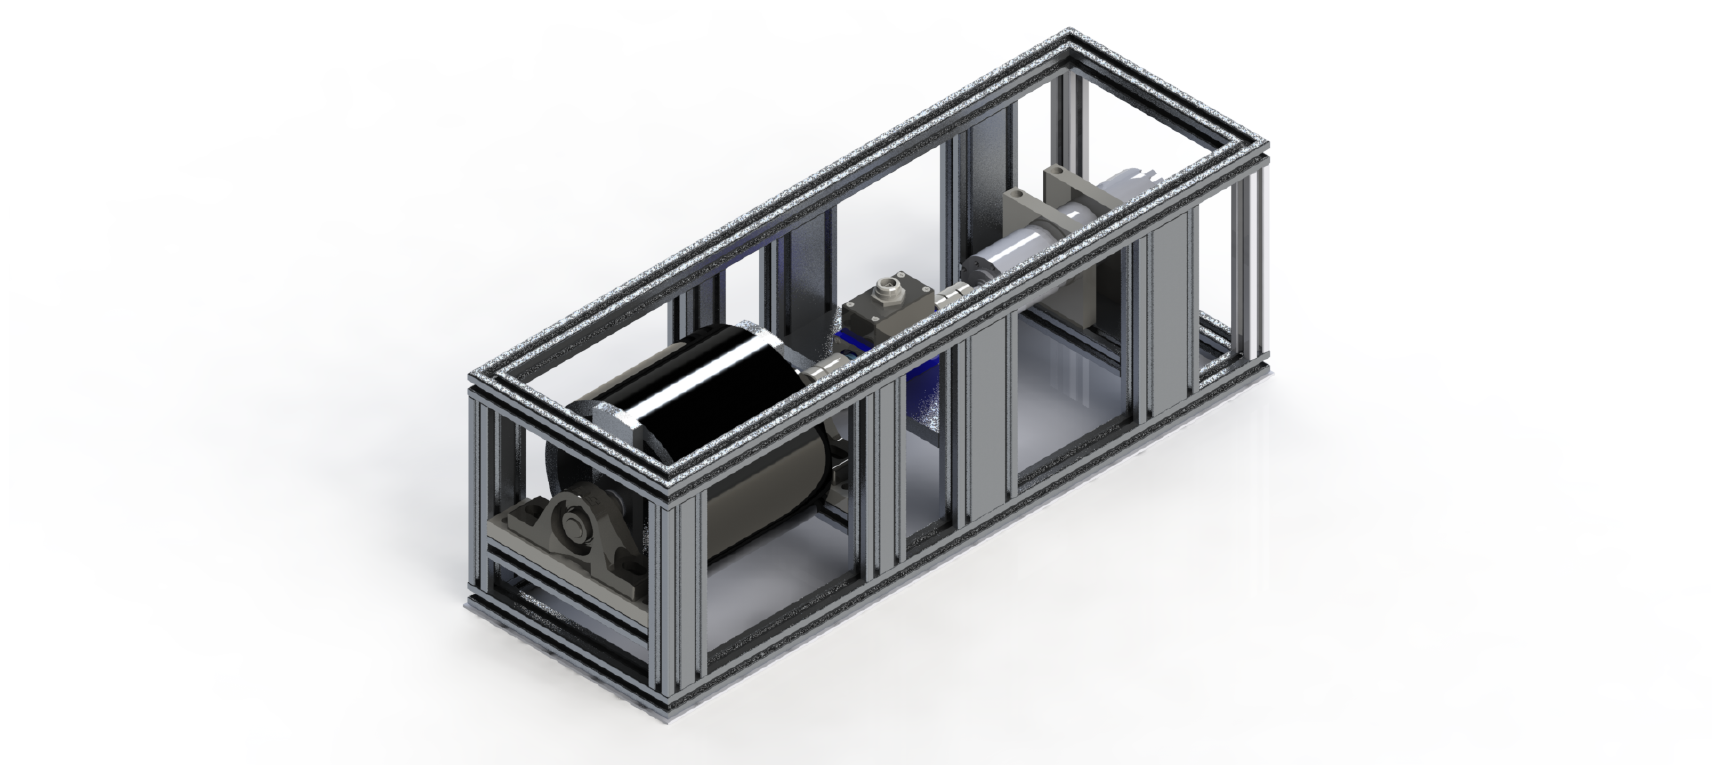
\includegraphics[width=0.5\linewidth]{Introduction/Model}
	\caption{Computer generated model of the system}
	\label{fig:System_model}
\end{figure}

\section{System description}
The primary purpose of the system is to measure the performance of an electrically propulsed car. The system has been designed with 'AU2' in mind, but can also be used to test individual motors; as long as they meet the specifications.

The performance is tested in order to optimize the propulsion-algorithm in the car's motor controller. Testing is done by placing the car on top of the dynamometer and connecting the car's battery to the measurement-system. The performance is measured as the amount of electrical power from the battery which is directly converted to the mechanical energy which spins the car's wheel.

During the test the system will collect data from the test-drive and send it to the 'Rolling Road GUI' where the data will be displayed graphically. The user is also able to regulate the amount of torque required to spin the roll in the dynamometer, by using this GUI, which makes it possible to simulate an elevation.

A quick overview of the system is shown in \ref{fig:System_overview}. It should be noted that neither the GUI nor 'AU2' are part of this system, but are seperate systems, which are required for complete functionality.

\begin{figure}[H]
	\centering
	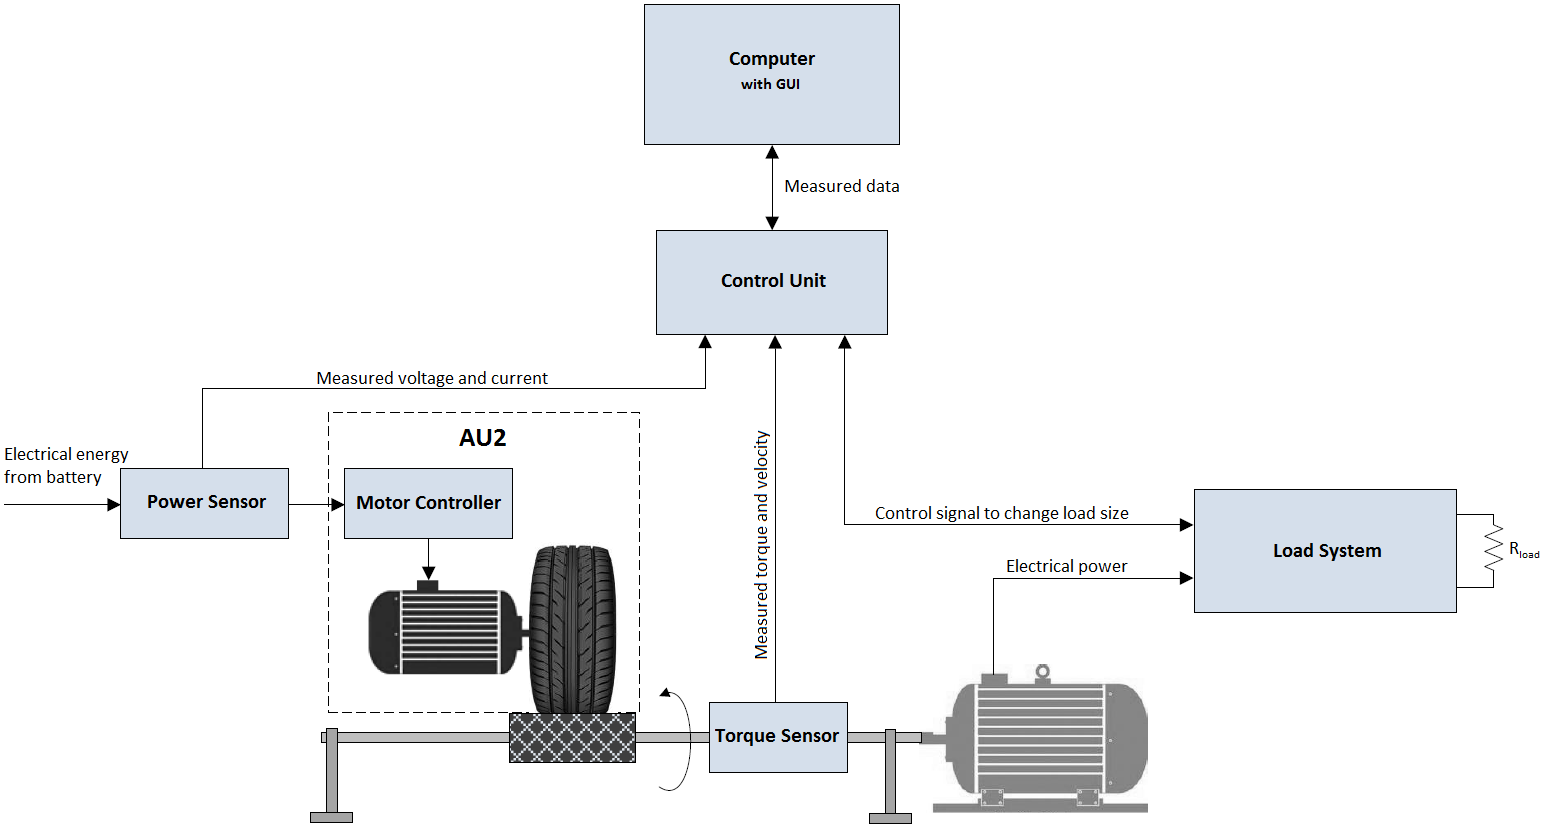
\includegraphics[width=1\linewidth]{Introduction/Overview}
	\caption{System overview}
	\label{fig:System_overview}
\end{figure}

\section{List of terms}
The following list explains the various terms which has been used to refer to certain parts or subsystems.
\begin{itemize}
	\item \textbf{AU2}\\
	Refers to the car which is being developed simultaneously as the dynamometer in order to optimize the car's performance. As the car and the dynamometer are being developed in parallel AU2 hasn't been tested during the writing-process of this documentation. Most calculations and tests in this documentations are instead based on Zenith33 (an earlier version of the car which was also developed to compete in the SHell Eco-Marathon).
	\item \textbf{SEM}\\
	Refers to the Shell Eco-Marathon which AU2 is designed to compete in.
	\item \textbf{GUI}\\
	Refers to the Rolling Road GUI which must loaded on a PC which is connected to Rolling Road, in order to get a visual representation of the measured data.
	\item \textbf{Load}\\
	Refers to the amount of torque which is required to spin the roll in the dynamometer.
	\item \textbf{PSoC}\\
	Refers to the CY8CKIT-059 PSoC 5LP Prototype Kit which is used as the Control Unit in the system.
	\item \textbf{Control-box}\\
	Refers to the electrical enclosure which contains the electrical systems - excluding the passive parts of the Load System. 
	\item \textbf{Load-plate}\\
	Refers the plate where the passive parts of the Load System (power resistors and super capacitor) are placed. These components are placed externaly due to their size and the generated heat.
\end{itemize}